The stepper component plays a central role in the propagation of track parameters. For inhomogeneous magnetic fields the trajectory of a chared particle cannot be expressed analytically. The stepper is responsible for the numerical integration of the equations of motion. Apart from that, it handles the transport of the Jacobian matrix and the covariance matrix for the track parameters which are used in the Kalman filter to fit tracks to measurements. As such, the stepper is a crucial component for track reconstruction.

Current stepper implementations in ACTS are based on a fourth-order Runge-Kutta-Nystrom integration, which is described in Section \ref{sec:into/reco/runge-kutta-nystrom}. While this is well established for track reconstruction, there is not a single best way to implement this to achieve optimal computational performance. Since the stepper is a performance critical component, developments have continued during the work on this thesis and will continue in the future.

This chapter dicusses the developments on the stepper component in ACTS during the work on this thesis. First, work on the ConstrainedStep is presented, which is a central helper class to deal with different step length requirements. Followed by a discussion on the adaptive step size technique, which is used to improve the performance of the numerical integration. Then, improvements on the EigenStepper are discussed which is a long standing stepper implementation in ACTS. Afterwards, the SympyStepper is introduced which is a novel stepper implementation in ACTS, conceptualized and implemented as part of this thesis. Finally, the computational cost of the time parameter is discussed.

\section{Reworking the ConstrainedStep}

ConstrainedStep is a helper class in ACTS to deal with different step length requirements. Currently, ACTS deals with 4 different types of step length request: \texttt{accuracy}, \texttt{navigator}, \texttt{actor}, and \texttt{user}. The \texttt{accuracy} limit is used to communicate an appropriate step length limit to achieve the requested integration accuracy target set by prior integration steps. The \texttt{navigator} limit holds the approximated distance to the next surface target. In case of overstepping the target, this can also be negative. The \texttt{actor} limit holds the approximate distance to the next abort condition, for example a trajectory path length limit or a target surface distance. Similar to the \texttt{navigator} limit, this can also be negative. The \texttt{user} limit is a user defined limit to restrict the step size to a given maximum.

A ConstrainedStep takes inputs from the different sources and provides a single step length. The step length is determined by the minimum of the \texttt{accuracy}, \texttt{navigator}, \texttt{actor}, and \texttt{user} limits, while overstepping resolution is always preferred over smaller absolute distances.

This class used to be quite involved and a central cause of problems for the propagation. Over multiple iterations it has been effectively rewritten during the work on this thesis, to be more robust and easier to understand. One major compilcation was the handling of the step direction inside the ConstrainedStep. The propagation can be done in both directions, forward and backward. During a backward propagation we might overstep a target. To resolve this we need to reverse direction, effectively stepping forward. This was all handled inside \texttt{ConstrainedStep} and resulted in failures in certain edge cases. In the new implementation this was simplified by removing the propagation direction sign from ConstrainedStep. With this change, it only deals with distances that have the propagation direction factored in. This is possible because the behavior of ConstrainedStep has to be symmetrical in forward and backward propagation.

Another major change was removing the sign of the \texttt{accuracy} limit. In rare cases the accuracy was set during overstep resolution which caused it to be negative. This effectively locked the step size resulting in a failed propagation due to reaching the step count limit. The new implementation decides the sign for the accuracy limit based on the \texttt{navigator} and \texttt{actor} limits.

\section{Adaptive step size}

Adaptive step size is a technique to improve the performance of the numerical integration given a certain accuracy target. The idea is to adjust the step size based on the local curvature of the trajectory. In regions of high curvature a smaller step size is used to resolve the trajectory more accuratly. In regions of low curvature a larger step size is used to accelerate the propagation and to limit the accumulation of machine precision errors.

This is done by computing an error estimate after each step of the numerical integration and comparing it to the requested accuracy target. If the error estimate is larger than the requested accuracy target the step size is reduced, otherwise it is increased.

A derivation of the expected error for the fourth-order Runge-Kutte-Nystrom is provided in \textcite{pub-2009-001} and only summarized here. The error estimate is given by

\begin{equation}
    \epsilon = h^2 \, \left\lVert \mathbf{k}_1 - \mathbf{k}_2 - \mathbf{k}_3 + \mathbf{k}_4 \right\rVert_1
\end{equation}

with the intermediate steps of the Runge-Kutta-Nystrom integration $\mathbf{k}_1$, $\mathbf{k}_2$, $\mathbf{k}_3$, and $\mathbf{k}_4$. Given the requested accuracy target $\tau$ and the used step length the next step length can be calculated with:\cite{pub-2009-001}\cite{numerical-recipes}

\begin{equation}
    h_{\text{next}} = h \, \left( \frac{\tau}{\epsilon} \right)^{1/4}
    \label{eq:dev/stepper/adaptive-step-size}
\end{equation}

The exponent of 1/4 is determined by the order of the Runge-Kutta-Nystrom integration.

Equation \ref{eq:dev/stepper/adaptive-step-size} is used after each step of the numerical integration to adjuste the step size. If the error estimate is too large, the step size is reduced and the step is reattempted. If the error estimate is too small, the step size is increased to accelerate the next integration step.

Since the error estimate can fluctuate, an upper and lower limit is imposed to the updated step size:

\begin{equation}
    \frac{1}{4} h < h_{\text{next}} < 4 h
\end{equation}

These limits ensure that the step size is not changed significantly. The accuracy condition is the following:

\begin{equation}
    \epsilon < 4 \tau
\end{equation}

If not satisfied the step is rejected and reattempted. The factor 4 gives some margin for the requested accuracy target and allows $\epsilon$ to fluctuate around $\tau$ without immediately rejecting steps.

The adaptive step size technique was implemented in ACTS during the work on this thesis and tested with the EigenStepper.

\begin{figure}[ht]
    \centering
    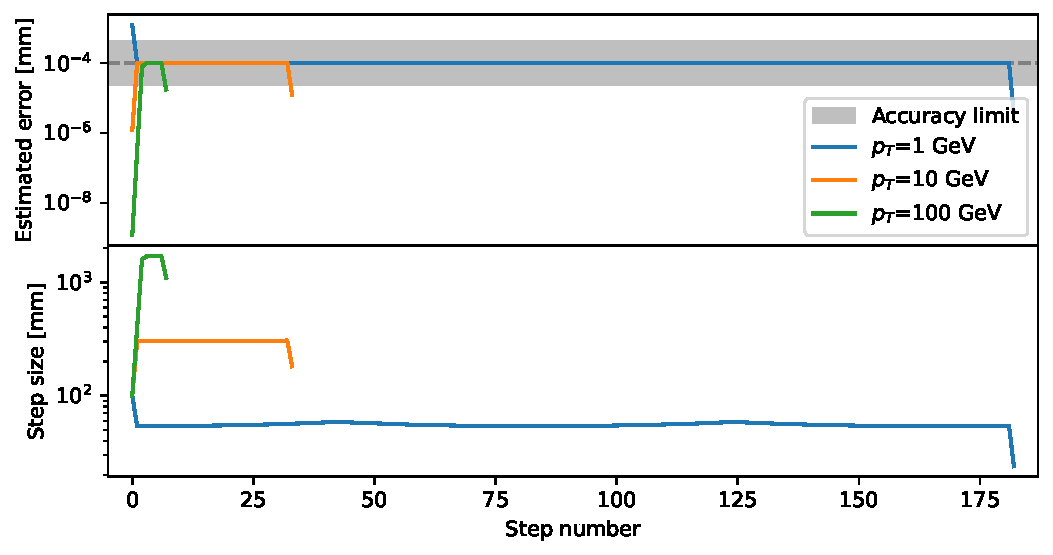
\includegraphics[width=1.0\textwidth]{parts/2_developments/05_stepper-developments/figures/adaptive_step_size_error.pdf}
    \caption{Error estimate and step size as a function of integration steps with different transverse momenta in a 2 T magnetic field propagated with $\theta=\pi/4$ for 10 m. The gray band indicates the requested accuracy limits.}
    \label{fig:dev/stepper/adaptive-step-size}
\end{figure}

Figure \ref{fig:dev/stepper/adaptive-step-size} shows the error estimate and the step size as a function of integration steps with different transverse momenta in a 2 T magnetic field propagated with $\theta=\pi/4$ for 10 m. The initial step size is set to 100 mm and the stepper successfully adapts the step size to stay close to the requested accuracy target. Tracks with high transverse momenta are followed with fewer steps and larger step sizes which accelerates the propagation. The last step has a smaller size and error as the path length of 10 m is reached with a smaller step size.

% pt=1GeV, B=2T, s=5m, cov=true
% without adaptive step size; just halfing if too big
% 13:29:52    SympyStepper   INFO      propagating 20000 tracks with pT = 1GeV in a 2T B-field
% 13:29:54    SympyStepper   INFO      Execution stats: 20000 runs of 1 iteration(s), 267.9ms total, 13.3340+/-0.0037µs per run, 13334.000+/-3.747ns per iteration
% 13:29:54    SympyStepper   INFO      average path length = 5000mm
% 13:29:54    SympyStepper   INFO      average number of steps = 192
% 13:29:54    SympyStepper   INFO      step efficiency = 0.984615
% with adaptive step size
% 13:31:45    SympyStepper   INFO      propagating 20000 tracks with pT = 1GeV in a 2T B-field
% 13:31:47    SympyStepper   INFO      Execution stats: 20000 runs of 1 iteration(s), 212.0ms total, 10.5830+/-0.0022µs per run, 10583.000+/-2.150ns per iteration
% 13:31:47    SympyStepper   INFO      average path length = 5000mm
% 13:31:47    SympyStepper   INFO      average number of steps = 144
% 13:31:47    SympyStepper   INFO      step efficiency = 0.986301

\begin{table}[ht]
    \centering
    \begin{tabular}{ccc}
        \hline
        \textbf{Strategy} & \textbf{Steps} & \textbf{Rel. time} \\
        \hline
        Half & 192 & 1.00 \\
        Adaptive & 144 & 0.79 \\
        \hline
    \end{tabular}
    \caption{Number of steps and relative CPU time for tracks with a transverse momentum of 1 GeV in a 2 T magnetic field propagated with $\theta=0$ for 5 m with different step size strategies.}
    \label{tab:dev/stepper/adaptive-step-size}
\end{table}


Table \ref{tab:dev/stepper/adaptive-step-size} shows the number of steps and the relative CPU time for tracks with a transverse momentum of 1 GeV in a 2 T magnetic field propagated with $\theta=0$ for 5 m with different step size strategies. \textit{Half} means that the step size is simply divided by 2 if the error estimate is too large. In this syntetic benchmark the adaptive step size strategy reduces the number of steps by 25\% and the CPU time by 21\%.

We should note that this is rather an upper limit for the performance improvement. The propagation inside a detector will not always allow to set the step size to its optimal value, as the navigation will usually require a smaller step size to resolve the geometry of the detector.

\section{EigenStepper}
\label{sec:dev/stepper/eigen}

The \texttt{EigenStepper} is a long standing stepper implementation in ACTS with the goal of being readable, maintainable and fast. It uses the C++ Eigen library for linear algebra operations which is the de facto standard. The math was once derived by hand and then transcribed into C++ code.

The EigenStepper has an extension mechanism, mainly to deal with vacuum and dense material stepping, but also to allow for potential future applications. Extensions are collected in a list and can bid for their priority in the given environment. An Auctioneer decides which extension is used for the current step based on the priority. The choosen extension is then used to calculate the intermediate steps of the Runge-Kutta-Nystrom integration and, in case of covariance transport, the transport Jacobian.

While the EigenStepper implementation is arguably doing well in terms of readability and maintainability, the extension mechanism diminishes these qualities. The Runge-Kutta-Nystrom integration is scattered between the stepper and the extensions which makes it hard to follow. To improve the situation, the EigenStepper was simplified during the work on this thesis. Instead of dealing with a list of extensions, only a single extension can now be provided. With that, the dense extension explicitly falls back to the default extension, if no volume material is present. This solved complications discovered during the work on the dense material propagation described in Chapter \ref{ch:dev/dense}, more specifically in Section \ref{sec:dev/dense/eigen}.

\section{SympyStepper}
\label{sec:dev/stepper/sympy}

\begin{itemize}
    \color{red}
    \item motivation
    \item comparison of EigenStepper, AtlasStepper, SympyStepper approach
    \item how is this done
\end{itemize}

The \texttt{SympyStepper} is a novel stepper implementation in ACTS, conceptualized and implemented as part of this thesis. It is based on generated code from the symbolic math library \texttt{SymPy}. The motivation for this stepper was to improve CPU performance while keeping or improving the readable representation of the mathematics.

The \texttt{EigenStepper} uses the C++ Eigen library for linear algebra operations which results in readable and hopefully fast code, as the library is sort of a de facto standard for linear algebra in C++ and supports vectorization. There are still a few weeknesses in terms of readability and maintainability with this implementation which is discussed in Section \ref{sec:dev/dense/eigen}. However, it was observed that the \texttt{AtlasStepper} is significantly faster than the \texttt{EigenStepper}. The \texttt{AtlasStepper} is based on the long standing Athena STEP algorithm and does not rely on any external libraries. The math operations are decomposed by hand and optimized for performance. This indeed results in fast code but is also practically unreadable and impossible to maintain. For example introducing a time parameter in the \texttt{AtlasStepper} would be significantly more involved than in the \texttt{EigenStepper}. It was attempted to improve the performance of the \texttt{EigenStepper} but turned out to be quite difficult and potentially reducing again readability and maintainability.

The \texttt{SympyStepper} can be thought of as the midpoint between the \texttt{EigenStepper} and the \texttt{AtlasStepper}. The stepper math is written in Python using the \texttt{SymPy} library. This allows for high level linear algebra operations while also deriving the linear error propagation from the Runge-Kutta-Nystrom integration. Apart from that we can use common subexpression elimination to simplify the math upfront and reduce the number of operations. Another big advantage is that we can encode known values and symmetries which will automatically result in simplified terms and fewer operations. Known values can be zeros in Jacobians we know from the beginning. We can also make use of the symmetry of the covariance matrix to avoid duplicate work. These kinds of simplifications are not possible with Eigen. Finally, we can generate C++ code from the \texttt{SymPy} expressions which can be used in the ACTS stepper implementation. The generated code is not meant to be readable but fast, can be thought of as binary code produced by a compiler and could be generated by a build system during the compilation of ACTS.

\section{The cost of the time parameter}

As mentioned before, the track parametrization is not customizable in ACTS. As such, the time parameter will always be present, even if it is not needed. This is the case for the ATLAS ITk detector which does not provide timing information. Since track reconstruction is a performance critical task, and the time parameter requires additional operations, the cost attached to it has to be evaluated.

Given the situation the current situation in ACTS, it is not easy to estimate this cost and any shortcuts might skew the results. For this reason the time parameter was consistently removed from ACTS in a separate branch and the performance difference was measured. Using the \texttt{EigenStepper} the performance was measured to be 10\% faster without the time parameter. This is a significant improvement and shows that the time parameter is indeed costly even if it is not used. However, after the implementation of the \texttt{SympyStepper} the impact was measured to be below 1\%. This suggests that the \texttt{SympyStepper} is indeed able to optimize the math operations to a high degree as the time parameter adds mostly zeros in derivatives for the linear error propagation.
